
\section{Séance 1}

\begin{exo}
Construisez un graphe simple et connexe sur $8$ sommets tel que chaque sommet est contenu dans exactement trois ar\^etes. Pouvez-vous faire la m\^eme chose avec $9$ sommets?
\end{exo}

Les sommets d'un graphe à un nombre pair de sommets sont de degré impair. Voici donc un exemple pour $n=8$.

\begin{figure}[!h]
\centering
\scalebox{.825}{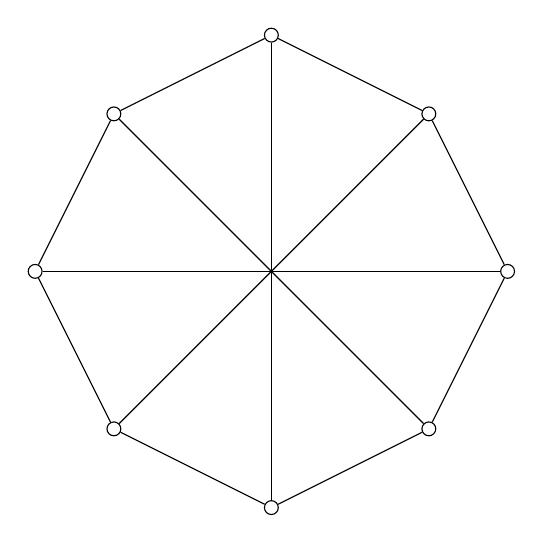
\begin{tikzpicture}

\tikzstyle{every node}=[circle, draw, fill=white, inner sep=0pt, minimum size=5pt]

\node (v2) at (0,0) {};
\node (v3) at (2,-1) {};
\node (v1) at (-2,-1) {};
\node (v8) at (-3,-3) {};
\node (v4) at (3,-3) {};
\node (v7) at (-2,-5) {};
\node (v5) at (2,-5) {};
\node (v6) at (0,-6) {};
\draw (v1) -- (v2) -- (v3) -- (v4) -- (v5) -- (v6) -- (v7) -- (v8) -- (v1);
\draw (v2) edge (v6);
\draw  (v5) edge (v1);
\draw  (v8) edge (v4);
\draw  (v7) edge (v3);
\end{tikzpicture}}
\end{figure}

Le nombre d'arêtes est donc de 12 ( $ \frac{n*d(v)}{2} = \frac{8*3}{2} = 12$) 

Pas possible pour n=9 car $ \frac{n*d(v)}{2} = \frac{9*3}{2} \cancel{\in} \N $

%-----------------------------------------------------------------

\begin{exo}
Dans un groupe de personnes, il y a toujours deux individus qui connaissent exactement le m\^eme nombre de membres du groupe.
\begin{enumerate}
\item Formalisez cette propri\'et\'e dans le vocabulaire des graphes.
\item D\'emontrez cette propri\'et\'e (par l'absurde).
\end{enumerate}
\end{exo}

\begin{enumerate}
\item Soit $\Gamma$ un graphe à n sommets. $\exists u,v \in V(\Gamma)$ tq $deg(u)=deg(v)$
\item Par l'absurde: Supposons que $\cancel{\exists}{} e_{1}, e_{2}: deg(e_{1}) = deg(e_{2})$. 

Les degrés sont tous compris entre 0 et n-1 (c'est à dire qu'on a un sommet pour chaque degré). Il existe donc un sommet qui est isolé (celui de degré 0) et un sommet qui est relié à ``tous'' les autres sommets (celui de degré n-1), ce qui est impossible.
\end{enumerate}

%-----------------------------------------------------------------

\begin{exo}
Soit $n\geq 2$ et soit $G$ un graphe simple avec $2n$ sommets et $n^2+1$ ar\^etes. Montrez par récurrence que $G$ contient un triangle.
\end{exo}

<MISSING>

%-----------------------------------------------------------------

\begin{exo}
Soit $G$ un graphe simple avec $2p$ sommets. On suppose que le degr\'e de chaque sommet est au moins \'egal \`a $p$. D\'emontrez que ce graphe est connexe.
\end{exo}

Démontrons par l'absurde: Supposons que le graphe ne soit pas connexe.

Soient x et y deux sommets tels qu'il n'existe pas de chemin entre x et y. Vu que $\forall v: deg(v)\geq p$, x a au moins p voisins (et y aussi). Les voisins de x sont différents des voisins de y, sinon il existerait un chemin entre x et y.

Le graphe est donc composé de $\underbrace{1+p}_{\text{x et ses voisins}}+\underbrace{1+p}_{\text{y et ses voisins}} = 2p+2$ sommets. Ceci est impossible, car l'énoncé dit que le graphe est composé de 2p sommets.

%-----------------------------------------------------------------

\begin{exo}
Soit $G$ un graphe simple.
\begin{enumerate}
\item On suppose que $G$ est connexe et que $x$ est un sommet de $G$ de degr\'e $1$. Prouvez que $G\setminus\{x\}$ est connexe.
\item D\'eduisez-en que, si $G$ est connexe et $|V(G)|=n\geq 2$, alors $G$ contient au moins $n-1$ ar\^etes.
\end{enumerate}
\end{exo}

<MISSING>

%-----------------------------------------------------------------

\begin{exo}
Donnez un graphe simple et connexe sur au moins $5$ sommets qui est:
\begin{itemize}
\item hamiltonien et eul\'erien;
\item hamiltonien et non eul\'erien;
\item non hamiltonien et eul\'erien;
\item non hamiltonien et non eul\'erien.
\end{itemize}
\end{exo}

\begin{figure}[!h]
\centering
\scalebox{.825}{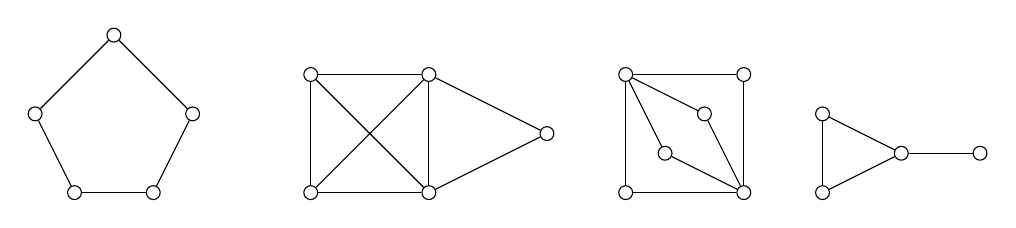
\begin{tikzpicture}
\tikzstyle{every node}=[circle, draw, fill=white, inner sep=0pt, minimum size=5pt]
\node (v2) at (-3.5,2) {};
\node (v1) at (-4.5,1) {};
\node (v3) at (-2.5,1) {};
\node (v5) at (-4,0) {};
\node (v4) at (-3,0) {};
\draw  (v1) edge (v2);
\draw  (v2) edge (v3);
\draw  (v3) edge (v4);
\draw  (v4) edge (v5);
\draw  (v5) edge (v1);
\node (v10) at (-1,0) {};
\node (v6) at (-1,1.5) {};
\node (v7) at (0.5,1.5) {};
\node (v9) at (0.5,0) {};
\node (v8) at (2,0.75) {};
\draw  (v6) edge (v7);
\draw  (v7) edge (v8);
\draw  (v8) edge (v9);
\draw  (v9) edge (v10);
\draw  (v10) edge (v6);
\draw  (v7) edge (v9);
\draw  (v9) edge (v6);
\draw  (v7) edge (v10);
\node (v11) at (3,1.5) {};
\node (v12) at (3,0) {};
\node (v13) at (3.5,0.5) {};
\node (v14) at (4,1) {};
\node (v15) at (4.5,1.5) {};
\node (v16) at (4.5,0) {};
\draw  (v11) edge (v12);
\draw  (v11) edge (v13);
\draw  (v11) edge (v14);
\draw  (v11) edge (v15);
\draw  (v15) edge (v16);
\draw  (v16) edge (v14);
\draw  (v16) edge (v13);
\draw  (v16) edge (v12);
\node (v17) at (5.5,0) {};
\node (v18) at (5.5,1) {};
\node (v19) at (6.5,0.5) {};
\node (v20) at (7.5,0.5) {};
\draw  (v17) edge (v18);
\draw  (v19) edge (v17);
\draw  (v19) edge (v18);
\draw  (v19) edge (v20);
\end{tikzpicture}}
\caption{Exemples pour chaque question, de gauche à droite.}
\end{figure}

Pour le quatrième, tout graphe contentant une feuille est une réponse possible.

%-----------------------------------------------------------------

\begin{exo}
Le graphe de la figure 2 est-il isomorphe \`a un (ou \`a plusieurs) des graphes de la figure 3?
\end{exo}

\begin{figure}[!h]
\centering
\scalebox{.825}{
\begin{tikzpicture}

\tikzstyle{every node}=[circle, draw, fill=white, inner sep=0pt, minimum size=5pt]

\node (a00) at (0,0) {};
\node (aleft) at (-1,0) {};
\node (aabove) at (0,1) {};
\node (adown) at (0,-1) {};
\node (aright) at (1,0) {};
\node (aright2) at (2,0) {};

\draw (a00) -- (aleft);
\draw (a00) -- (aright);
\draw (a00) -- (adown);
\draw (a00) -- (aabove);
\draw (aright) -- (aright2);
\end{tikzpicture}}
\caption{}
\end{figure}

\begin{figure}[!h]
\scalebox{.825}{
\begin{minipage}[t]{0.2\linewidth}
   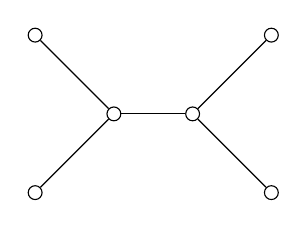
\begin{tikzpicture}
		\tikzstyle{every node}=[circle, draw, fill=white, inner sep=0pt, minimum size=5pt]

        \node (a00) at (0,0) {};
        \node (leftup) at (-1,1) {};
        \node (leftdown) at (-1,-1) {};
        \node (a01) at (1,0) {};
        \node (rightup) at (2,1) {};
        \node (rightdown) at (2,-1) {};

		\draw (a00) -- (leftup);
		\draw (a00) -- (leftdown);
		\draw (a00) -- (a01);
		\draw (a01) -- (rightup);
		\draw (a01) -- (rightdown);
	\end{tikzpicture}
\end{minipage}

\begin{minipage}[t]{0.2\linewidth}
   \begin{tikzpicture}
		\tikzstyle{every node}=[circle, draw, fill=white, inner sep=0pt, minimum size=5pt]

        \node (a0) at (0,0) {};
        \node (a1) at (1,0) {};
        \node (a0side) at (-1,0) {};
        \node (a0up) at (0,1) {};
        \node (a0down) at (0,-1) {};
        \node (a1side) at (2,0) {};
        \node (a1up) at (1,1) {};
        \node (a1down) at (1,-1) {};

		\draw (a0side) -- (a0) -- (a1) -- (a1side);
		\draw (a0up) -- (a0) -- (a0down);
		\draw (a1up) -- (a1) -- (a1down);

	\end{tikzpicture}
\end{minipage}

\begin{minipage}[t]{0.2\linewidth}
   \begin{tikzpicture}
		\tikzstyle{every node}=[circle, draw, fill=white, inner sep=0pt, minimum size=5pt]

        \node (a00) at (0,0) {};
		\node (a0up) at (0,1) {};
		\node (a0down) at (0,-1) {};
		\node (a0ddown) at (0,-2) {};
		\node (a0left) at (-1,1) {};
		\node (a0right) at (1,1) {};

		\draw (a0up) -- (a00) -- (a0down) -- (a0ddown);
		\draw (a00) -- (a0left);
		\draw (a00) -- (a0right);
	\end{tikzpicture}
\end{minipage}

\begin{minipage}[t]{0.2\linewidth}
	\hspace{-1cm}
   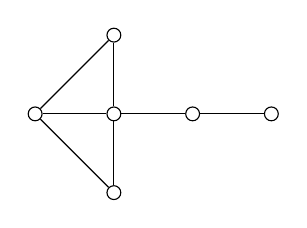
\begin{tikzpicture}
		\tikzstyle{every node}=[circle, draw, fill=white, inner sep=0pt, minimum size=5pt]

        \node (a00) at (0,0) {};
        \node (a0up) at (0,1) {};
        \node (a0down) at (0,-1) {};
        \node (a0left) at (-1,0) {};
        \node (a0right) at (1,0) {};
        \node (a0rright) at (2,0) {};

		\draw (a0left) -- (a00) -- (a0right) -- (a0rright);
		\draw (a0up) -- (a00) -- (a0down);
		\draw (a0up) -- (a0left) -- (a0down);
	\end{tikzpicture}
\end{minipage}

\begin{minipage}[t]{0.2\linewidth}
   \begin{tikzpicture}
		\tikzstyle{every node}=[circle, draw, fill=white, inner sep=0pt, minimum size=5pt]

        \node (a00) at (0,0) {};
		\node (a0up) at (0,1) {};
		\node (a0down) at (0,-1) {};
		\node (a0ddown) at (0,-2) {};
		\node (a0left) at (-1,-1) {};
		\node (a0right) at (1,0) {};

		\draw (a0up) -- (a00) -- (a0down) -- (a0ddown);
		\draw (a00) -- (a0left);
		\draw (a0down) -- (a0right);
	\end{tikzpicture}
\end{minipage}

\begin{minipage}[t]{0.2\linewidth}
   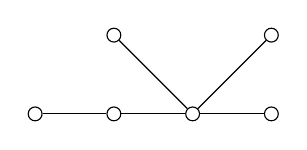
\begin{tikzpicture}
		\tikzstyle{every node}=[circle, draw, fill=white, inner sep=0pt, minimum size=5pt]

        \node (a00) at (0,0) {};
		\node (a0left) at (-1,0) {};
		\node (a0right) at (1,0) {};
		\node (a0rright) at (2,0) {};
		\node (a0upleft) at (0,1) {};
		\node (a0upright) at (2,1) {};

		\draw (a0left) -- (a00) -- (a0right) -- (a0rright);
		\draw (a0upleft) -- (a0right) -- (a0upright);
	\end{tikzpicture}
\end{minipage}}
\caption{}
\end{figure}

Le troisième et le sixième.

\newpage

%-----------------------------------------------------------------

\begin{exo}
Les graphes suivants sont-ils isomorphes~? (Ne vous contentez pas d'une justification approximative: essayez de d\'emontrer rigoureusement vos affirmations.)
\end{exo}

\begin{figure}[!h]
\centering

\begin{minipage}[t]{0.2\linewidth}
	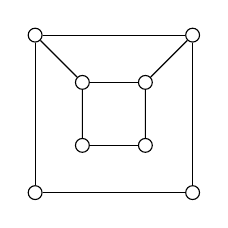
\begin{tikzpicture}[scale=0.4]
		\tikzstyle{every node}=[circle, draw, fill=white, inner sep=0pt, minimum size=5pt]

		\node (v6) at (-3.5,2.5) {};
		\node (v5) at (-5.5,2.5) {};
		\node (v8) at (-5.5,0.5) {};
		\node (v7) at (-3.5,0.5) {};
		\node (v1) at (-7,4) {};
		\node (v2) at (-2,4) {};
		\node (v4) at (-7,-1) {};
		\node (v3) at (-2,-1) {};
		\draw  (v1) edge (v2);
		\draw  (v3) edge (v2);
		\draw  (v4) edge (v3);
		\draw  (v1) edge (v4);
		\draw  (v5) edge (v6);
		\draw  (v6) edge (v7);
		\draw  (v7) edge (v8);
		\draw  (v8) edge (v5);
		\draw  (v5) edge (v1);
		\draw  (v6) edge (v2);
	\end{tikzpicture}
\end{minipage}
\hspace{1.5cm}
\begin{minipage}[t]{0.2\linewidth}
	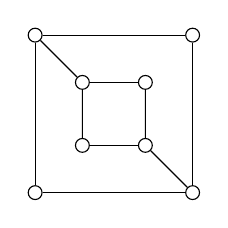
\begin{tikzpicture}[scale=0.4]
		\tikzstyle{every node}=[circle, draw, fill=white, inner sep=0pt, minimum size=5pt]

		\node (v6) at (-3.5,2.5) {};
		\node (v5) at (-5.5,2.5) {};
		\node (v8) at (-5.5,0.5) {};
		\node (v7) at (-3.5,0.5) {};
		\node (v1) at (-7,4) {};
		\node (v2) at (-2,4) {};
		\node (v4) at (-7,-1) {};
		\node (v3) at (-2,-1) {};
		\draw  (v1) edge (v2);
		\draw  (v3) edge (v2);
		\draw  (v4) edge (v3);
		\draw  (v1) edge (v4);
		\draw  (v5) edge (v6);
		\draw  (v6) edge (v7);
		\draw  (v7) edge (v8);
		\draw  (v8) edge (v5);
		\draw  (v5) edge (v1);
		\draw  (v7) edge (v3);
	\end{tikzpicture}
\end{minipage}
\caption{}
\end{figure}%

Non isomorphes. 

\begin{figure}[!h]
\centering

\begin{minipage}[t]{0.2\linewidth}
   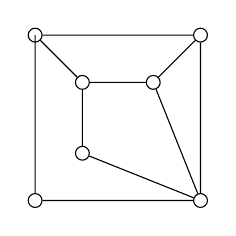
\begin{tikzpicture}[scale=0.6]
		\tikzstyle{every node}=[circle, draw, fill=white, inner sep=0pt, minimum size=5pt]

        \node (v6) at (0,0) {};
		\node (v7) at (1.5,0) {};
		\node (v5) at (0,-1.5) {};
		\node (v1) at (-1,1) {};
		\node (v2) at (2.5,1) {};
		\node (v4) at (-1,-2.5) {};
		\node (v3) at (2.5,-2.5) {};
		\draw (v1) -- (v2) -- (v2) -- (v3) -- (v3) -- (v4) -- (v4) -- (-1,1);
		\draw (v5) -- (v6) -- (v6) -- (v7) -- (v7) -- (v3) -- (v3) -- (v5) -- (v6) -- (v1);
		\draw (v2) -- (v7);
	\end{tikzpicture}
\end{minipage}
\hspace{1.5cm}
\begin{minipage}[t]{0.2\linewidth}
   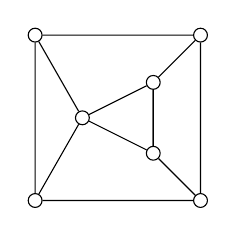
\begin{tikzpicture}[scale=0.6];
		\tikzstyle{every node}=[circle, draw, fill=white, inner sep=0pt, minimum size=5pt]

        \node (v1) at (-0.5,0.25) {};
		\node (v2) at (-1.5,2) {};
		\node (v5) at (-1.5,-1.5) {};
		\node (v6) at (1,1) {};
		\node (v3) at (2,2) {};
		\node (v7) at (1,-0.5) {};
		\node (v4) at (2,-1.5) {};
		\draw (v2) -- (v3) -- (v4) -- (v5) -- (v2) -- (v1) -- (v6) -- (v7) -- (v1) -- (v5);
		\draw (v3) -- (v6) -- (v7) -- (v4);

	\end{tikzpicture}
\end{minipage}
\caption{}
\end{figure}

Non isomorphes (il existe un sommet de degré 2 dans le graphe de gauche, tandis qu'aucun sommet du graphe de droite est de degré 2).

\begin{figure}[!h]
\centering
\begin{minipage}[t]{0.2\linewidth}
   \begin{tikzpicture}[scale=2]
   		\node[draw=none,minimum size=3cm,regular polygon,regular polygon sides=7] (a) {};

		\foreach \x in {1,2,...,7}
			\draw[fill=white,inner sep=0pt, minimum size=5pt] (a.corner \x) circle (1.5pt);
		  
		\draw (a.corner 1) -- (a.corner 2) -- (a.corner 3) -- (a.corner 4) -- (a.corner 5) -- (a.corner 6) -- (a.corner 7) -- (a.corner 1);
		\draw (a.corner 2) -- (a.corner 7) -- (a.corner 5) -- (a.corner 3) -- (a.corner 1) -- (a.corner 6) -- (a.corner 4) -- (a.corner 2) ;

	\end{tikzpicture}
\end{minipage}
\hspace{1.5cm}
\begin{minipage}[t]{0.2\linewidth}
   \begin{tikzpicture}[scale=2]
		\node[draw=none,minimum size=3cm,regular polygon,regular polygon sides=7] (a) {};

		\foreach \x in {1,2,...,7}
  			\draw[fill=white,inner sep=0pt, minimum size=5pt] (a.corner \x) circle (1.5pt);

		\draw (a.corner 1) -- (a.corner 5) -- (a.corner 2) -- (a.corner 6) -- (a.corner 3) -- (a.corner 7) -- (a.corner 4) -- (a.corner 1);
		\draw (a.corner 1) -- (a.corner 2) -- (a.corner 3) -- (a.corner 4) -- (a.corner 5) -- (a.corner 6) -- (a.corner 7) -- (a.corner 1);


	\end{tikzpicture}
\end{minipage}
\caption{}
\end{figure}

Isomorphes.